\documentclass{article}

\usepackage{geometry}
\geometry{margin=2cm}
\usepackage{graphicx}
\usepackage{hyperref}
\usepackage{amsfonts}
\usepackage{caption}
\usepackage{subcaption}

\hypersetup{colorlinks=true, linkcolor=blue, urlcolor=blue}
\urlstyle{same}
\begin{document}
	
	\author{Aayush Arya}
	\date{(Submitted: \today)}
	\title{}
	
	\maketitle
	
	\hrule
	\begin{center}
		PHY366 Lab Report\\
		Practical(s): 4 \& 5 \quad Registration No.: 11912610 \quad Section: G2903
	\end{center}
	\hrule
	
	\section*{Aim}
	To study the low-pass, high-pass, band-pass and band-reject active filters.
	
	\section*{Methods}
	
	We simulate our operational amplifier circuit on the \textsc{MultiSim} platform. In this section, we quickly summarize the circuit schematics and in \nameref{sect:results}, we discuss the frequency response received and how that compares with expectations.
	
	For simplicity, in both high and low-pass filters, we have consistently used $R=1k\Omega$ and $C = 1\mu F$. This configuration corresponds to a cutoff frequency of $f_c = 159.2$ Hz.\\
	
	\textbf{Low Pass Filter}
	
	
	\begin{figure}[h!]
		\centering
		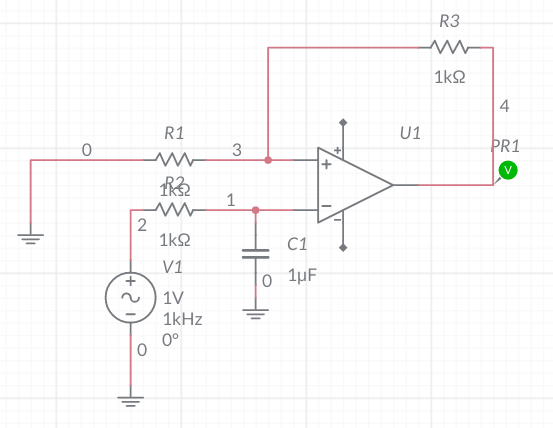
\includegraphics[width=0.6\textwidth]{low_pass_circuit}
		\caption{Low-pass filter circuit}
		\label{fig:low_pass_circuit}
	\end{figure}
	
	\textbf{High Pass Filter}\\
	
	The high-pass filter circuit illustrated in Figure \ref{fig:high_pass_circuit} is available publicly at \url{https://www.multisim.com/content/krAnsJD3FhLvUGbCkkjTk8/low-pass-filter/open/}.\\
	
	\begin{figure}[h!]
		\centering
		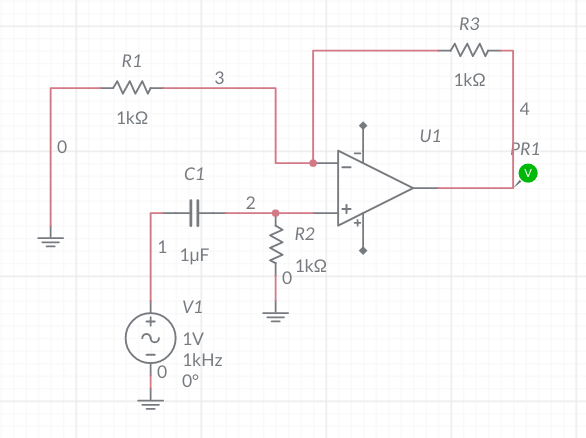
\includegraphics[width=0.5\textwidth]{high_pass_circuit}
		\caption{High pass filter circuit}
		\label{fig:high_pass_circuit}
	\end{figure}
	
	\pagebreak \textbf{Band Pass Filter}\\
	
	We configured the filter such that the maxima occurs at $1.59$ kHz (as opposed to 159.2 Hz in previous cases). Circuit available at \url{https://www.multisim.com/content/GL9t3YLGo2bemhTcSeW6Qn/band-pass-filter/open/}.\\
	
	\textbf{Band Reject Filter}
	
	\begin{figure}[h!]
		\centering
		\begin{subfigure}{0.48\textwidth}
			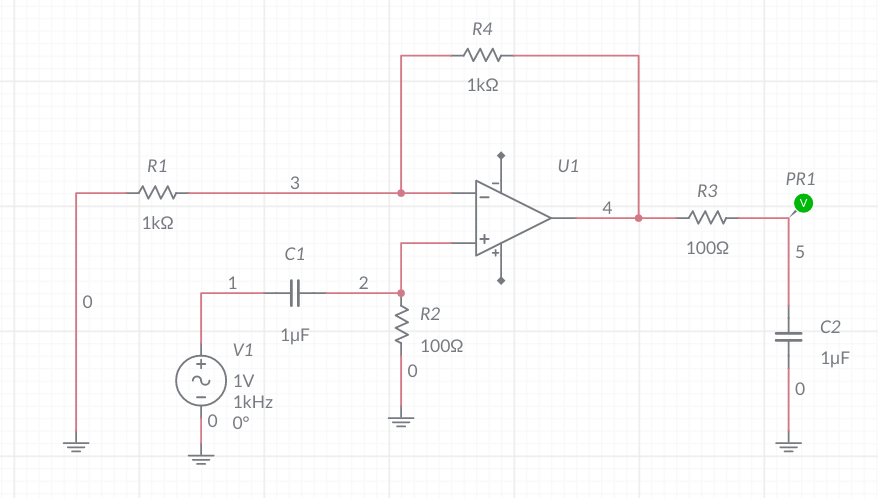
\includegraphics[width=\textwidth]{band_pass_circuit}
			\caption{Band pass}
		\end{subfigure}
		
		\begin{subfigure}{0.48\textwidth}
			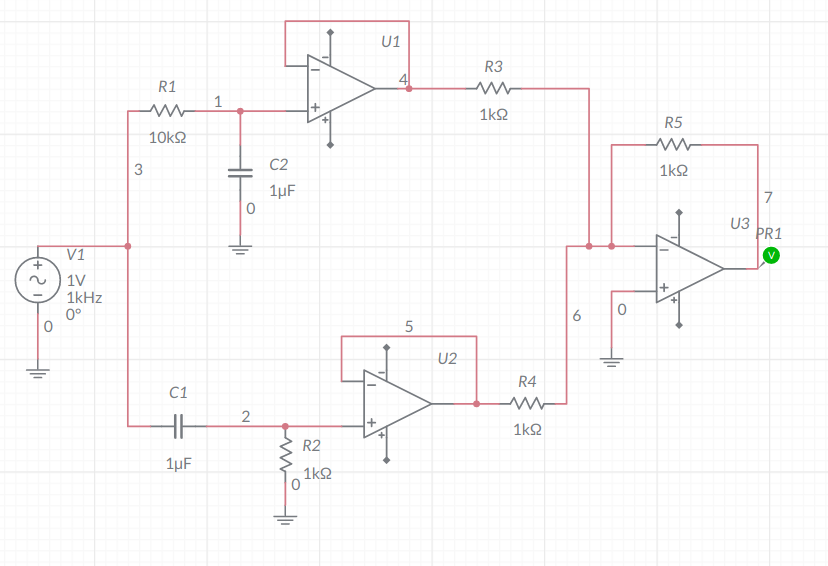
\includegraphics[width=\textwidth]{band_reject_schematic}
			\caption{Band reject}
		\end{subfigure}
		\caption{Band pass and reject filters}	
	\end{figure}

	\pagebreak
	
	\section*{Results and Discussion}
	\label{sect:results}
	
	We show the frequency response profile we obtained for the high and low pass filters in Figure \ref{fig:high_low}. The important features of these circuits can be understood based on the following fashion:\\
	
	\begin{figure}[!h]
		\centering
		\begin{subfigure}{0.8\textwidth}
			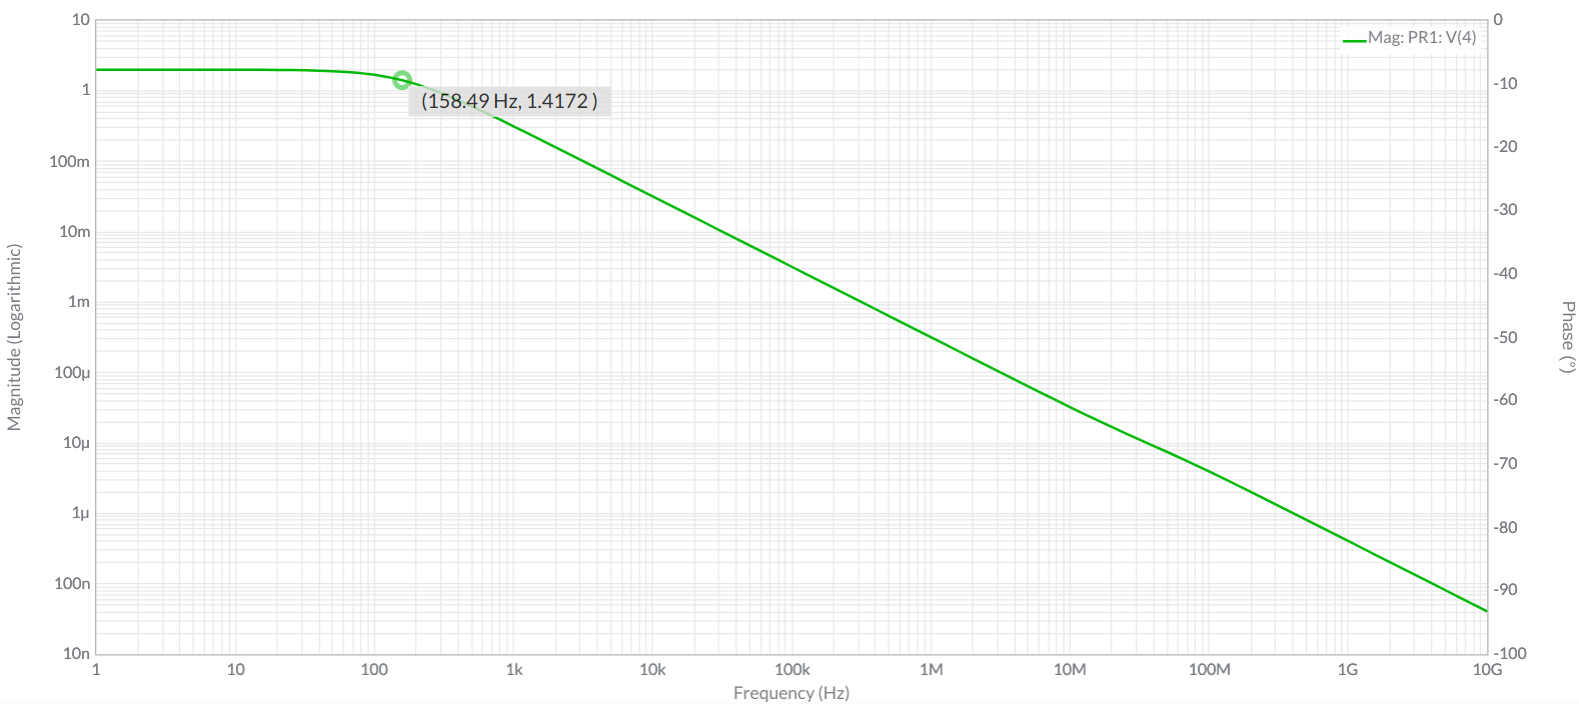
\includegraphics[width=\textwidth]{low_pass_response}
			\caption{Low-pass filter frequency response}
		\end{subfigure}
		
		\begin{subfigure}{0.8\textwidth}
			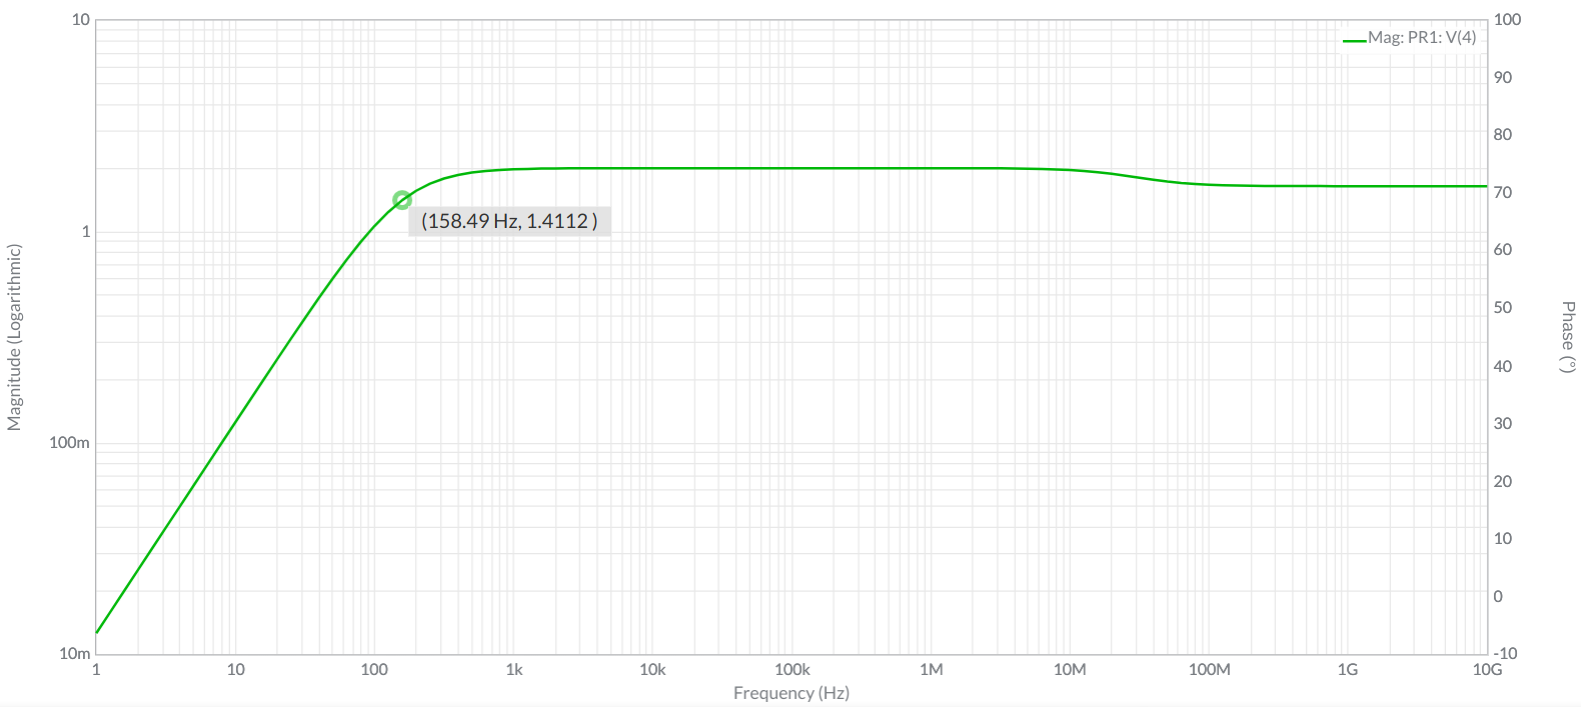
\includegraphics[width=\textwidth]{high_pass_response}
			\caption{High-pass filter frequency response}
		\end{subfigure}
		\caption{Frequency response of high- and low-pass filter circuits.}
		\label{fig:high_low}
	\end{figure} 

	We expect a low pass filter to allow lower frequencies unimpeded while higher ones get attenuated. The characteristic frequency beyond which the attenuation starts to become significant is the {\it cutoff frequency}. For a low-pass filter circuit $$ V_o = \frac{V_{in}}{\sqrt{ \left( \frac{f}{f_{cl}} + 1  \right)^2}}$$ where the cutoff frequency $$f_{cl} = \frac{1}{2\pi RC}$$
	
	for a high pass-filter on the other hand.
	$$ V_o = \frac{V_{in}}{ \sqrt{\left( 1 + \frac{f_{ch}}{f}\right)^2} } $$
	
	The cutoff frequency for the configuration $R=1k\Omega$ and $C=1\mu$F turns out to be $f_c = 159.2 \mathrm{Hz}$ for both high and low pass configurations. At this frequency, we expect our amplitude to drop to $1\sqrt{2} \simeq 0.707$ times.

	It it indeed evident in Figure \ref{fig:high_low} that at roughly the cutoff frequency, the voltage drops to $0.707\times 2 \simeq 1.414$ V.\\
	
	We show the frequency dependence of the output for the band pass and band-reject filters in Figure \ref{pass_reject}.
	
	\begin{figure}
		\centering
		\begin{subfigure}{0.8\textwidth}
			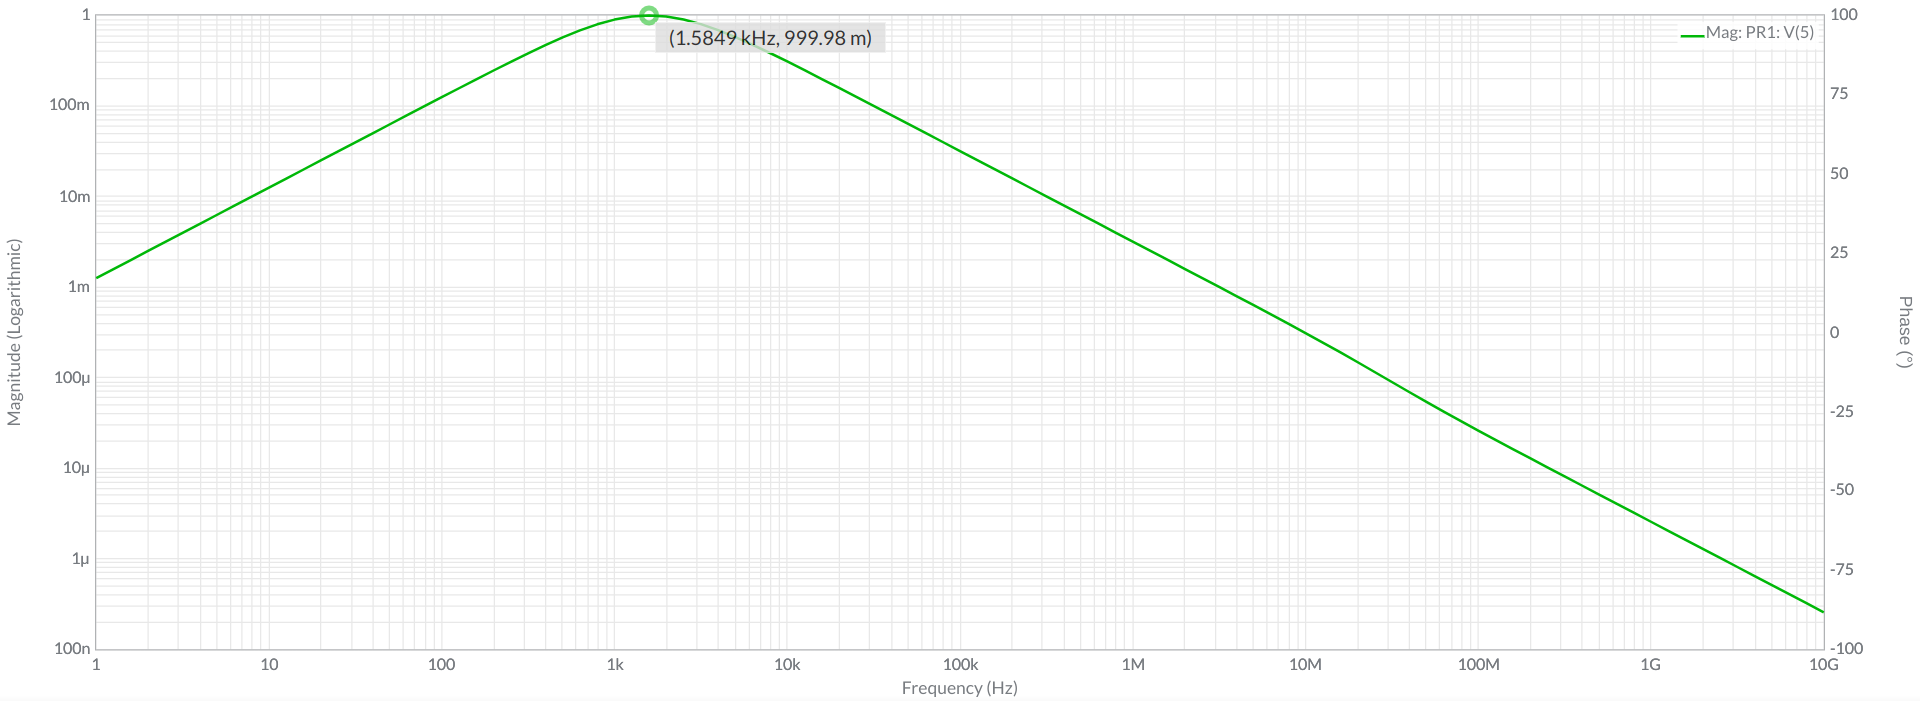
\includegraphics[width=\textwidth]{band_pass_response}
			\caption{Band pass}
		\end{subfigure}	
	
		\begin{subfigure}{0.7\textwidth}
			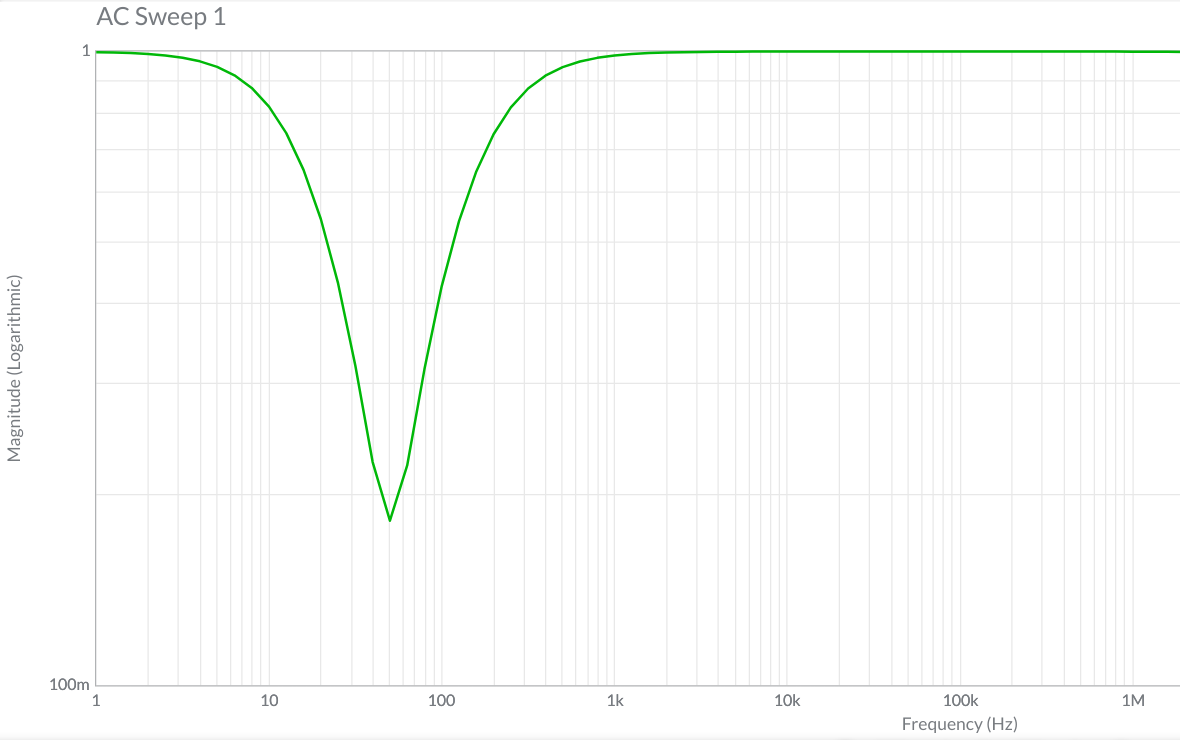
\includegraphics[width=\textwidth]{band_reject_response}
			\caption{Band reject}
		\end{subfigure}
		\caption{Frequency dependence for the band pass and band-reject filter}
		\label{pass_reject}
	\end{figure}

	The maxima of the bandpass filter is expected at $f_{max} = \sqrt{f_{ch}f_{cl}}$. Since the cutoff $f_{ch} = f_{cl} = 1.59$ kHz. The result is as expected in Figure \ref{pass_reject}
	
	
\end{document}